%!TEX root = ../graduate-work.tex

\section{Результаты}

\subsection{Конфигурация экспериментов}

Экспериментальная проверка предложенного способа оценки качества русскоязычных радиологических отчётов проводилась на наборе данных из 100 исследований. В экспериментах использовалась одна фиксированная русскоязычная клиническая компонента, а также 35 текстовых и 10 визуально-текстовых оценок. После сопоставления текстовых и визуально-текстовых компонент по общему суффиксу, соответствующему переводчику и режиму использования терминологии при подготовке английской версии отчёта, было сформировано 70 допустимых конфигураций. На каждом шаге вложенной кросс-валидации способ автоматически выбирал одну из 70 троек вида
\[
(\text{ru-компонента},\ \text{text-компонента},\ \text{img-компонента}),
\]
после чего для неё подбирал веса линейного смешивания.

Оценка выполнялась по схеме вложенной кросс-валидации с параметрами
\[
K_{\mathrm{outer}} = 5,\qquad K_{\mathrm{inner}} = 5.
\]
Подбор весов осуществлялся перебором по сетке на симплексе с шагом
\[
h = 0.05.
\]

\subsection{Количественные результаты}

Главным результатом эксперимента является оценка качества предложенного подхода на внешних тестовых разбиениях. Среднее значение целевой функции $J_{\mathrm{outer}} = -\tau$ по пяти внешним фолдам составило $\overline{J}_{\mathrm{outer}} = 0.5927$, стандартное отклонение -- 0.1491, а 95\%-й доверительный интервал -- [0.4621;\ 0.7234].

Поскольку в работе используется величина $J = -\tau\!\left(S, y\right)$, где \(S\) -- итоговая оценка качества отчёта, а \(y\) -- число ошибок, полученный результат соответствует средней корреляции Кендалла \(\overline{\tau}_{\mathrm{outer}} = -0.5927\).
Таким образом, между итоговой оценкой качества и числом ошибок наблюдается устойчивая отрицательная связь: чем выше итоговая оценка, тем, как правило, меньше число ошибок в отчёте. Эта зависимость показана на рис.~\ref{fig:final_score_vs_errors}.

\begin{figure}[ht]
    \centering
    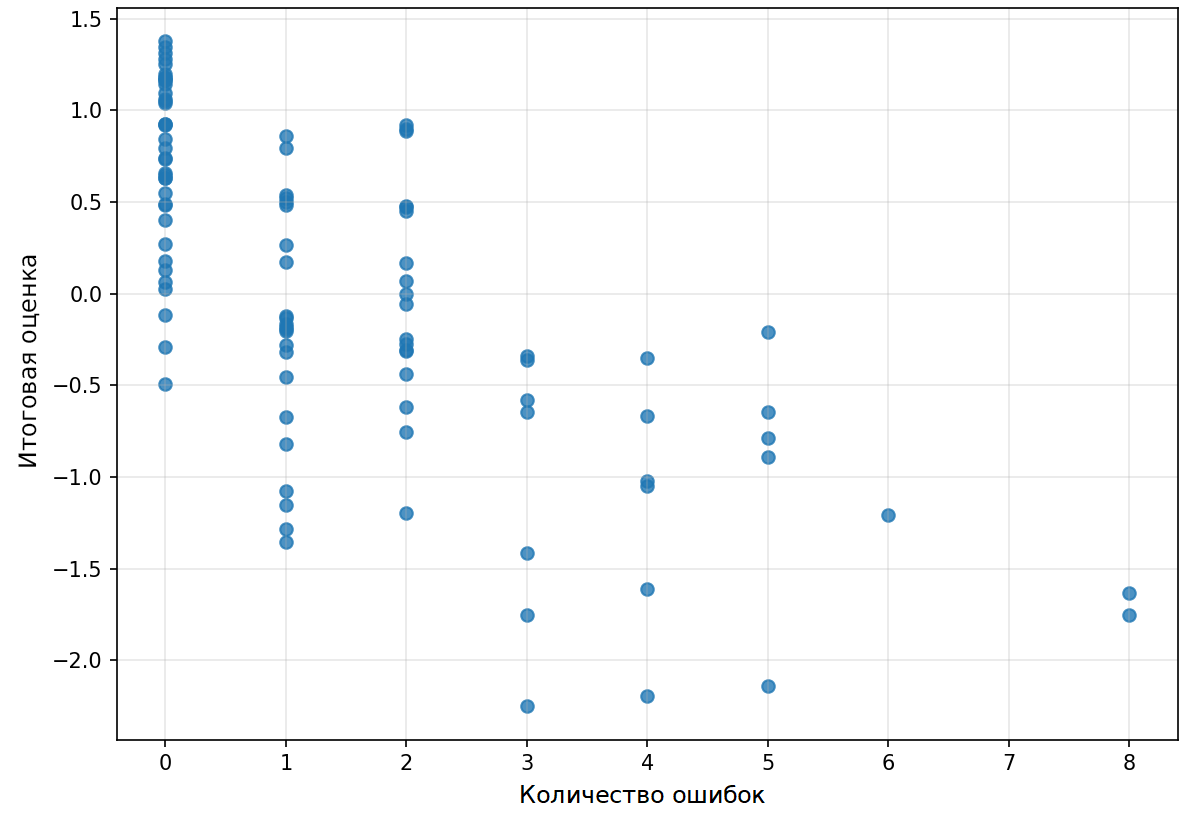
\includegraphics[width=0.8\textwidth]{images/plot_final_score_vs_errors.png}
    \caption{Связь итоговой оценки качества отчёта с числом ошибок на объединении внешних тестовых фолдов.}
    \label{fig:final_score_vs_errors}
\end{figure}

Значения \(J_{\mathrm{outer}}\) по отдельным внешним фолдам составили:
\[
0.5064,\quad 0.4265,\quad 0.7503,\quad 0.5296,\quad 0.7508.
\]
Разброс по фолдам заметен из-за малого объёма данных, что также иллюстрируется на рис.~\ref{fig:inner_vs_outer}, однако во всех случаях знак корреляции остается правильным, а сама связь между итоговой оценкой и числом ошибок остается отрицательной. В то же время доверительный интервал остается достаточно широким. Это связано с тем, что оценка строится всего по пяти внешним фолдам и по относительно небольшому набору из 100 объектов. Поэтому полученные результаты следует интерпретировать как подтверждение работоспособности предложенного способа оценки в условиях ограниченных данных, а не как окончательную и исчерпывающую оценку его качества на всех возможных русскоязычных радиологических корпусах.

\begin{figure}[ht]
    \centering
    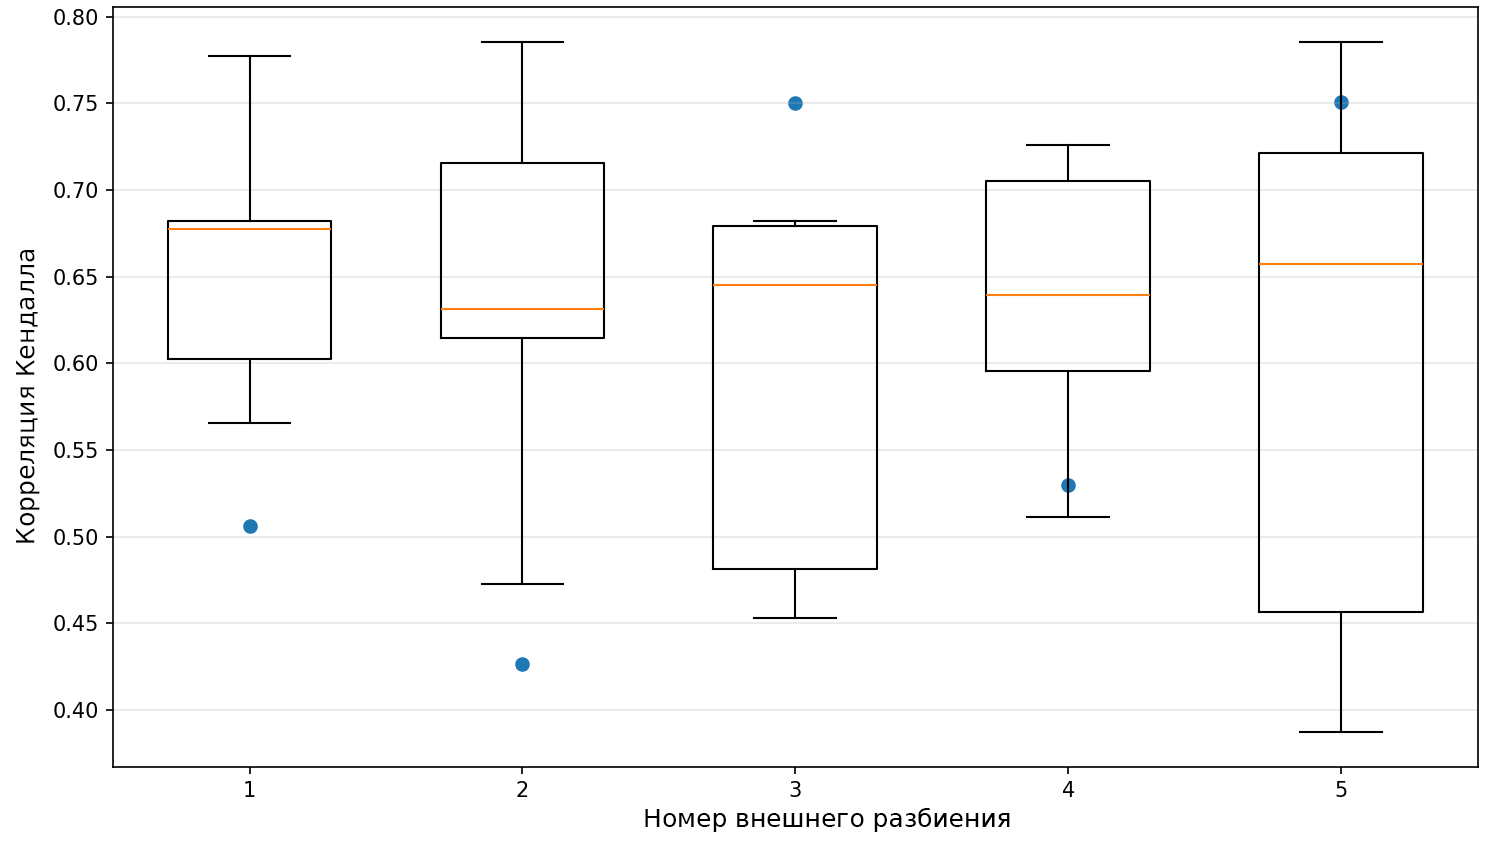
\includegraphics[width=0.8\textwidth]{images/plot_inner_selected_vs_outer_test.png}
    \caption{Сопоставление распределения значений целевой функции на внутренних валидационных разбиениях для выбранной конфигурации с её значением на соответствующем внешнем тестовом разбиении: ящичные диаграммы показывают разброс значений на внутренних разбиениях, отдельные точки -- значения на внешнем тестовом разбиении.}
    \label{fig:inner_vs_outer}
\end{figure}

% Во всех пяти внешних фолдах в качестве лучшей текстовой компоненты выбирался один и тот же тип сигнала -- косинусная близость текстовых представлений.

% Аналогичная устойчивость наблюдается и для визуально-текстовой компоненты. Во всех пяти внешних фолдах среди лучших конфигураций выбирались варианты семейства \texttt{img\_en\_biovilt\_*}. Следовательно, именно этот тип визуально-текстового сигнала оказался наиболее согласованным с экспертным числом ошибок на данном наборе данных.

% Если рассматривать используемые варианты перевода, то в трёх из пяти внешних фолдов была выбрана конфигурация с ключом \texttt{hy\_noterms}, в одном фолде -- \texttt{hy\_terms}, и еще в одном -- \texttt{medgemma\_noterms}. Конфигурации, связанные с \texttt{qwen}-переводом, среди лучших на внешних фолдах не появились.

Не менее важным результатом является распределение весов между тремя компонентами итоговой оценки качества. Средние значения весов по пяти внешним фолдам составили:
\[
\overline{w}_{\mathrm{ru}} = 0.11,\qquad
\overline{w}_{\mathrm{text}} = 0.59,\qquad
\overline{w}_{\mathrm{img}} = 0.30.
\]
% Распределение выбранных весов по внешним фолдам приведено на рис.~\ref{fig:weight_distribution}.

% \begin{figure}[ht]
%     \centering
%     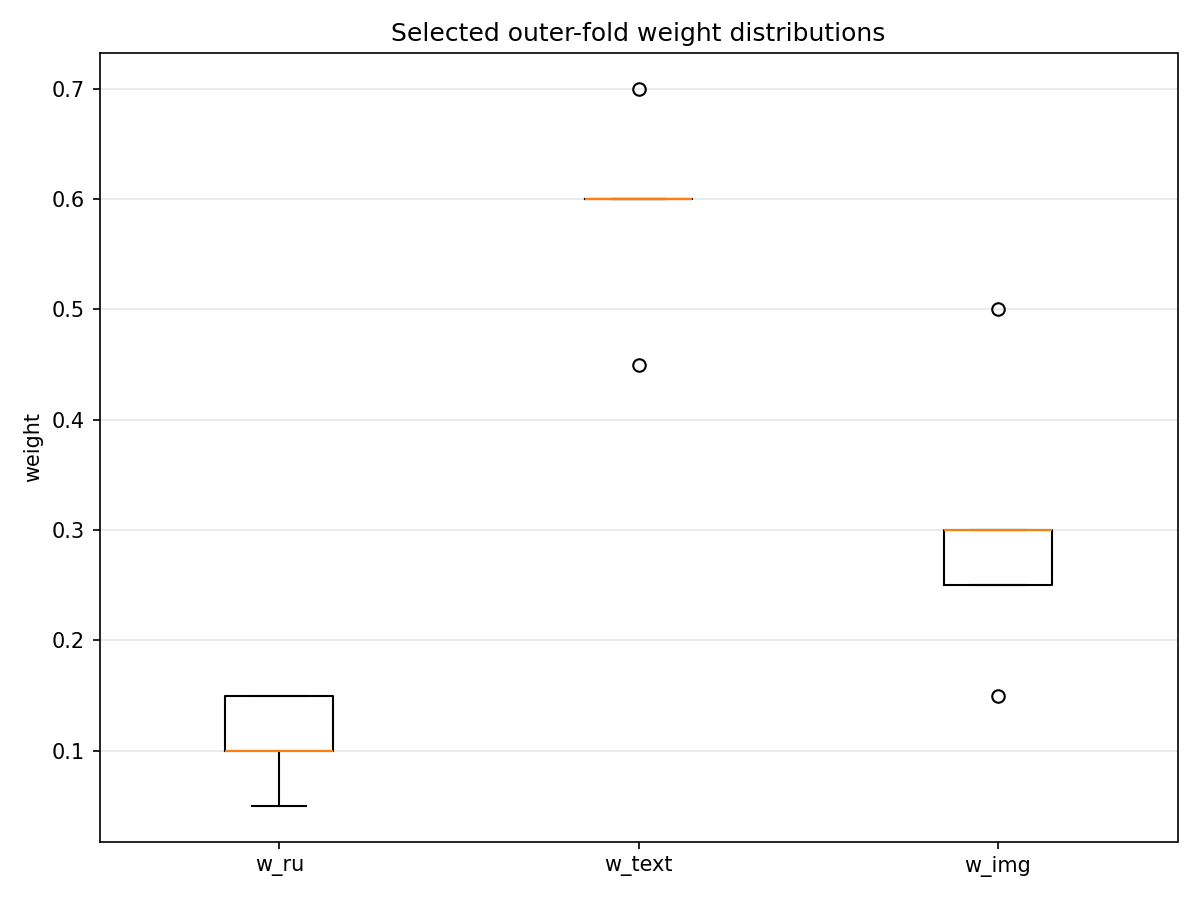
\includegraphics[width=0.8\textwidth]{images/plot_weight_distribution.png}
%     \caption{Распределение весов \(w_{\mathrm{ru}}\), \(w_{\mathrm{text}}\), \(w_{\mathrm{img}}\) выбранных на внешних фолдах для русскоязычной клинической, текстовой и визуально-текстовой компонент соответственно.}
%     \label{fig:weight_distribution}
% \end{figure}

Следовательно, наибольший вклад в итоговую оценку качества в среднем вносила текстовая компонента. Визуально-текстовая компонента также вносила существенный вклад, однако в среднем уступала текстовой. Русскоязычная клиническая компонента имела наименьший средний вес, но при этом сохранялась во всех выбранных решениях и давала интерпретируемый результат.

По отдельным фолдам веса изменялись в следующих диапазонах:
\[
w_{\mathrm{ru}} \in [0.05;\ 0.15],\qquad
w_{\mathrm{text}} \in [0.45;\ 0.70],\qquad
w_{\mathrm{img}} \in [0.15;\ 0.50].
\]

Полученные результаты подтверждают, что в условиях дефицита русскоязычных размеченных данных более целесообразно оценивать не один заранее зафиксированный способ, а всю адаптивную процедуру выбора конфигурации и весов. Внешняя вложенная кросс-валидация показывает, что такой подход позволяет устойчиво выявлять отрицательную связь между итоговой оценкой качества и числом ошибок, причём делает это без обучения новой крупной специализированной модели.

По результатам экспериментов можно сделать следующие выводы: предложенный способ оценки качества русскоязычных радиологических отчётов органов грудной клетки:
\begin{enumerate}
    \item корректно работает в условиях малого объёма данных;
    \item устойчиво сочетает три источника информации -- русскоязычный клинический, текстовый и визуально-текстовый;
    \item чаще всего опирается на текстовую семантическую близость как на основной сигнал;
    \item использует визуально-текстовую согласованность как значимую дополнительную компоненту;
    \item требует рассматривать результат именно как процедуру выбора, а не как одну универсальную фиксированную формулу.
\end{enumerate}

\subsection{Дальнейшее развитие}
В условиях дефицита размеченных данных обучение русскоязычной клинической текстовой модели с нуля невозможно. Поэтому была предложена методика оценки, состоящая из комбинации методов трёх семейств: русскоязычная большая языковая модель для интерпретации ошибок, отобранные на этапе предварительного сравнения методы сопоставления текста-кандидата с эталоном и с рентгенограммой, включающие предварительный машинный перевод на английский язык с последующим применением готовых англоязычных методов. Оценка качества работы самой методики производилась с помощью вложенной кросс-валидации, что позволило получить несмещённую оценку обобщающей способности подхода в целом.

Среди потенциальных путей совершенствования предложенной методики следует отметить возможную врачебную валидацию автоматического перевода набора данных. Другим перспективным направлением для будущих работ может стать доработка алгоритмов с учётом их соответствия российским стандартам написания рентгенологических отчётов. Это позволило бы лучше адаптировать подход под специфику отечественного здравоохранения и повысить его практическую значимость.